\hypertarget{tripoli-beyrouth-qadisha-sauxefda}{%
\section{Tripoli, Beyrouth, Qadisha,
Saïda}\label{tripoli-beyrouth-qadisha-sauxefda}}

\emph{Lundi 21 mai 2018}

\hypertarget{mapid}{}

La semaine dernière, nous avons poursuivi nos excursions depuis
Beyrouth.

La première a été la ville de Tripoli, au nord du Liban. On y trouve le
château Saint Gilles, initialement construit par les croisés, en très
bon état. Situé au sommet de la colline, il propose une belle vue sur la
ville et la côte. Nous y avons également visité un hammam vieux de 800
ans et restauré depuis sa fermeture dans les années 1970. Après avoir
traversé le dédale des ruelles du vieux souk, nous avons fini la journée
dans une des institutions de la ville : la pâtisserie Hallab où on a pu
déguster des douceurs locales...

\begin{figure}
\centering
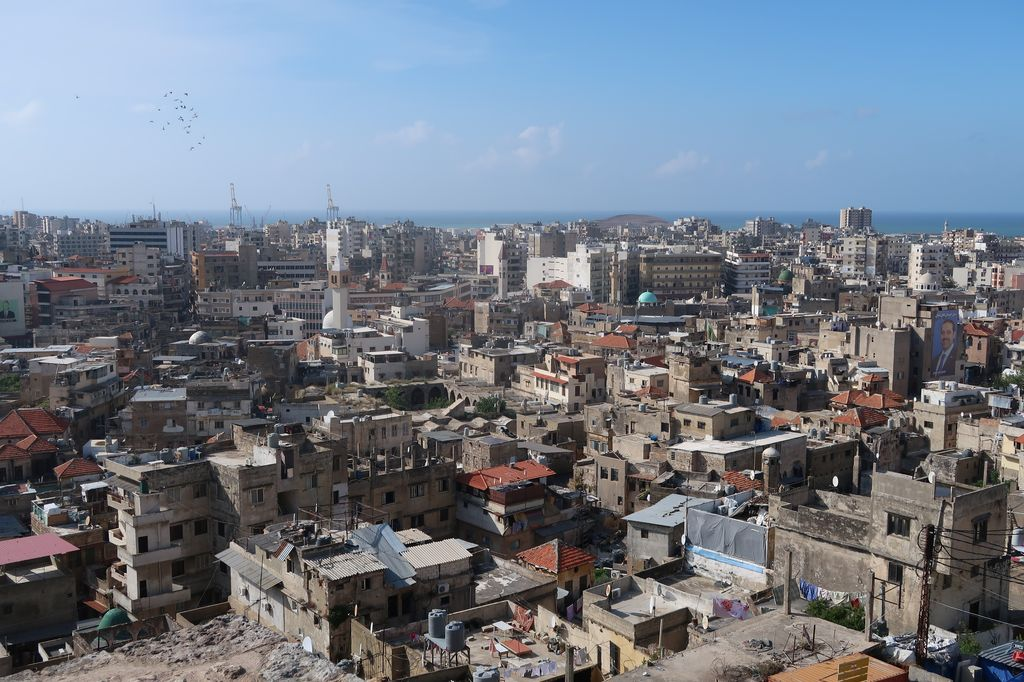
\includegraphics{images/20180521_tripoli.JPG}
\caption{Vue sur Tripoli depuis le château Saint Gilles.}
\end{figure}

Nous avons profité d'avoir un gîte à Beyrouth pour nous promener durant
plusieurs journées dans la ville. Que retenir de la capitale du Liban ?
Pour moi, c'est un mélange étonnant de routes serrées et de ruelles, de
voitures trop nombreuses, de promenades en bord de mer, d'immeubles
abandonnés, d'impacts de balles rebouchés ou non sur les façades, de
blocs d'appartement modernes et de villas somptueuses. On peut noter que
le centre ville a été reconstruit à neuf après les années de guerre
civile (1975 - 1990) et a une allure atypique et très propre de ce fait.
Nous avons également profité de l'agréable musée national qui nous a
permis de couvrir du regard les millénaires d'histoire du Liban, et du
musée de l'American University of Beirut qui est venu compléter cette
parenthèse dans le passé.

\begin{figure}
\centering
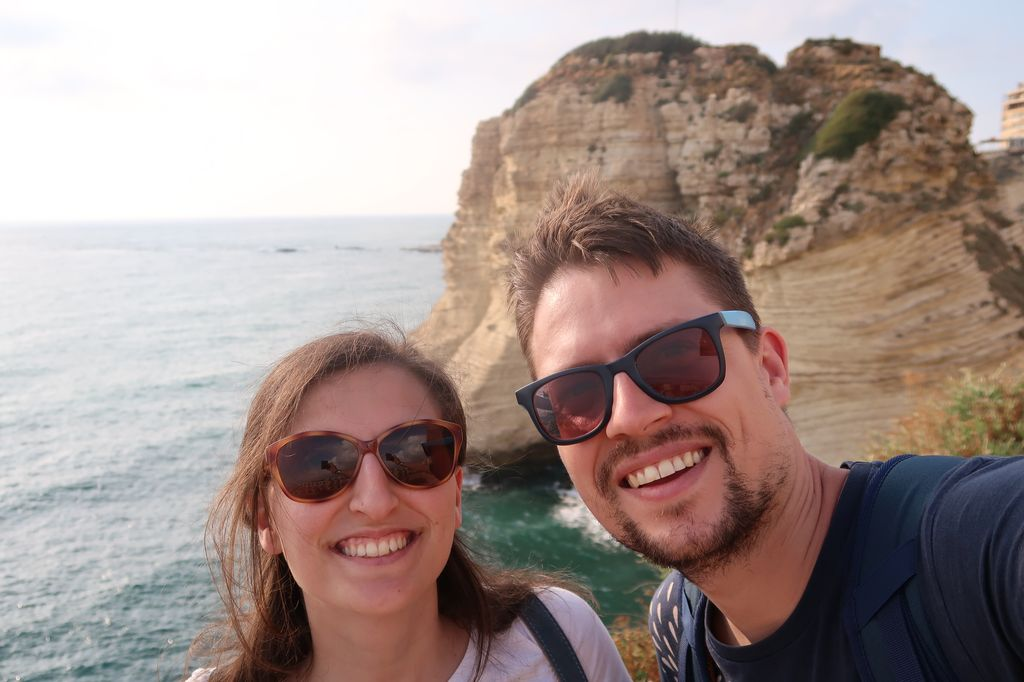
\includegraphics{images/20180521_Rausche.JPG}
\caption{Selfie devant l'une des vues touristiques de Beyrouth : le
rocher aux pigeons.}
\end{figure}

L'un des moments les plus agréables de cette semaine a été l'excursion
dans la "vallée sainte de Qadisha". Cette vallée porte une longue
histoire religieuse, ayant été tour à tour refuge de chrétiens
persécutés ou d'ermites, avec de nombreuses caves creusées dans la roche
ainsi que de nombreux monastères construits au fil des quinze derniers
siècles. Nous avons eu la chance de la visiter en présence d'un guide
français, "Monsieur Yves", qui nous a plus d'une fois surpris par la
profondeur de son érudition et sa connaissance pointue du lieu. Il nous
a emmené randonner dans la vallée, jusqu'à Hawqa où vit actuellement un
ermite, puis jusqu'au couvent de Qannoubine où vivent encore deux
religieuses. La marche est raide mais très belle et impressionnante. On
a du mal à imaginer les conditions d'accès à ces sanctuaires il y a
plusieurs centaines d'années, sans équipement si aménagements du
sentier.

\begin{figure}
\centering
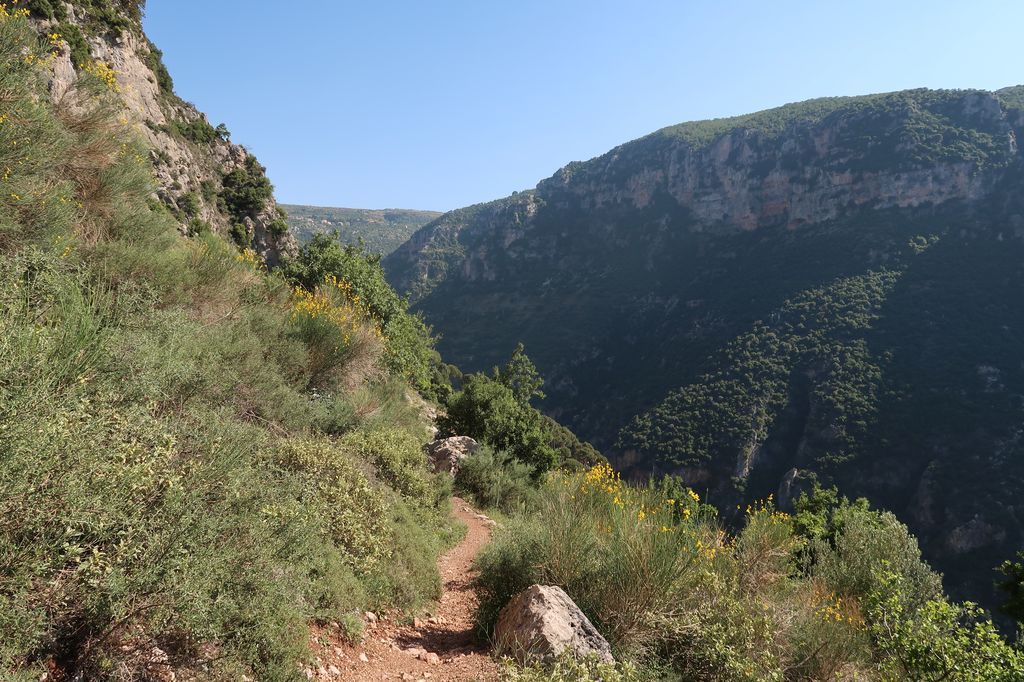
\includegraphics{images/20180521_qadisha.JPG}
\caption{La végétation dans la vallée de Qadisha.}
\end{figure}

Notre dernière excursion de la semaine nous a amené à Saïda, au sud de
Beyrouth. A ce sujet, il est intéressant de noter que l'on se déplace
facilement en bus au Liban, mais avec un certain nombre de différences
par rapport aux bus que j'ai l'habitude de prendre : absence d'arrêts
officiels (on peut monter à partir du moment où on fait signe au
chauffeur, y compris sur la bande d'arrêt d'urgence de l'autoroute), pas
d'horaires définis, prix non affichés... A Saïda, nous avons trouvé une
petite ville avec un souk typique, une citadelle marine de l'époque des
croisés (encore eux !) ainsi qu'un musée du savon plutôt bien fait. Note
pour plus tard : visiter une ville à prédominance musulmane le premier
jour du Ramadan n'est pas une mince affaire lorsqu'il s'agit de se
restaurer ;)

Enfin, nous avons également ajouté à la liste des sanctuaires visités
celui de Saint Charbel, l'un des saints libanais les plus connus.

Bon, il commence à faire un peu trop chaud à Beyrouth, on retourne plus
en altitude pour nos derniers jours ici :)

\emph{Florian et Elida}
